\chapter{Implementation}

\chapterintro{
  This chapter details a proof-of-concept implementation of Cloud-SAP architecture.
}

\section{Introduction}
Previous chapters detailed requirements that a self-manageable platform oriented toward Quality-of-Service assurance should comply with. Beside this, reference architecture known as Cloud-SAP was introduced. This chapter in turn highlights key elements of a proof-of-concept implementation of Cloud-SAP. Noticeably, our implementation is by all means not exhaustive and merely intends to prove that presented architecture successfully tackles raised challenges. Hence, we implemented only following subset of managers specified by Cloud-SAP:
\begin{itemize}
  \item Autonomic container manager
  \item Autonomic stack manager
  \item Autonomic cloud instance manager
  \item Autonomic cloud federation manager
\end{itemize}

Apart from that, we implemented minimal viable modules that is monitoring, analysis, planning and execution. For example, we based analysis solely on threshold model, discarding more advanced techniques that uses prediction mechanisms.

\section{Overview}
As previous section indicates, key elements of discussed implementation are as follows: autonomic container manager, autonomic stack manager, autonomic cloud instance manager, autonomic cloud federation manager. Taking their role in service deployment into account, we grouped them into auto-scaling and cloud brokerage subsystems. High level overview of system, including its internal and external elements is depicted in figure \ref{fig:hlo-implementation}. Diagram \ref{fig:csap-layers-subsystem} illustrates thee relationship between Cloud-SAP managers and above-mentioned subsystems. 

\begin{figure}[!ht]
  \begin{center}
    \includegraphics[width=\textwidth]{chapter-implementation/hlo-implementation}
  \end{center}
  \caption{High level system overview}
  \label{fig:hlo-implementation}
\end{figure}

\begin{figure}[!ht]
  \begin{center}
    \includegraphics{chapter-implementation/csap-layers-subsystem}
  \end{center}
  \caption{System parts and their relation with autonomic managers}
  \label{fig:csap-layers-subsystem}
\end{figure}

As one can see, our implementation is composed by following parts:
\begin{asparaenum}
 \item[\textbf{Auto-scaling subsystem}] Auto-scaling subsystem supervises service's life cycle, monitoring it and enacting scaling actions when necessary. It is concentrated on all service's aspects: containers, stacks and application instances thus it is in fact a group of autonomic managers composed by container, stack and cloud instance managers.

 \item[\textbf{Cloud brokerage subsystem}] Brokerage subsystem groups components that together mediates between cloud providers. In particular, it consists of:
  \begin{itemize}
   \item Cloud broker - probes cloud providers and selects best offer according to a given policy. In Cloud-SAP model, it plays a role of orchestrating autonomic manager, that is, autonomic cloud federation manager.
   \item Cloud client - delegates service provisioning request to a cloud broker.
  \end{itemize}
 
 \item[\textbf{Cloud provider}] External system that manages a group of resource such as computing nodes, storage and networking typologies. Particularly, it is able to deploy, shutdown, migrate and monitor containers. Although Cloud-SAP is utterly cloud provider independent, our implementation is solely focused on OpenNebula that uses OpenVZ as a hypervisor. We selected OpenNebula due to its simplicity, flexibility and our expertise in managing it. Choosing hypervisor, we were compelled to select one that is based on lightweight containers due to theirs flexibility in scaling as previously advocated. OpenVZ was a natural choice due to its maturity and our familiarity within it.
 
 \item[\textbf{Application provider}] An entity that is interested in application scaling and deployment. It can be represented by a human being as well as by an external system.
\end{asparaenum}

With those information in mind, we can illustrate overall architecture, components and communication protocols on deployment diagram \ref{fig:hlo-deployment}. Successive sections portrays in detail specified elements.

\section{Technology stack overview}
This section aims to give a brief outline of technologies that were used in this implementation with an endeavour to justify our choice. The chosen solutions are grouped according to their presence in appropriate subsystems.

\begin{itemize}
  \item Cloud brokerage subsystem
    \begin{asparaenum}
    \item[\textbf{Web Services/HTTP}] Communication between a client and a cloud broker is done by the usage of \emph{web services} over \emph{http} protocol. The cloud broker for a given client exposes a \emph{RESTful} API for the deployment of a service. The web service accepts \emph{JSON}-encoded messages, which comprises the name of a service and specification of each stack comprising it. The example of such a message can be found in listing \ref{lst:service-spec-test-deployment-time}.

      The reason we chose this technology is because of its simplicity, maturity and great support from Ruby platform. The other solutions that could be used in place of this one include some message-oriented middleware standards such as AMQP or JMS, other standards that facilitate communications among systems/components such as CORBA, and other such as RMI or RPC. Some of the aforementioned technologies had been eliminated once we chose Ruby as the language the platform would be implemented in. This is because of their platform-specific nature, e.g. JMS requires the system to be written in Java.

    \item[\textbf{AMQP}] Being able to communicate in an asynchronous, more scalable and loosely coupled way between a cloud broker and different cloud instance managers representing cloud providers requires the usage of message-oriented middleware. In our case we decided to use \emph{Advanced Message Queuing Protocol}as this standard is mature and its support in Ruby is solid.

      This communication channel is used in the implementation to 
      \begin{inparaenum}[a)]
      \item get offers from cloud providers for a given service and
      \item commission the cloud provider to deploy a service.
      \end{inparaenum}

    \item[\textbf{SQLite}] For the persistence layer there was a need for a lightweight database engine that would have good support in Ruby platform. Possible choices included some nonrelational solutions, such as Redis, and more traditional, relational ones, such as SQLite. We chose the latter as the drivers for \emph{DataMapper}, an ORM library, have better support in Ruby.
    \end{asparaenum}

  \item Auto-scaling subsystem
    \begin{asparaenum}
    \item[\textbf{OpenNebula}]
    \item[\textbf{OpenNebula AppFlow/AppStage ?}]
    \item[\textbf{Chef}]
    \item[\textbf{OpenVZ (drivers)}]
    \end{asparaenum}
\end{itemize}

\newpage
\begin{figure}[!ht]
  \begin{center}
    \includegraphics{chapter-implementation/hlo-deployment}
  \end{center}
  \caption{System's deployment diagram}
  \label{fig:hlo-deployment}
\end{figure}

\section{Cloud brokerage subsystem}


\section{Auto-scaling subsystem}

\subsection{Objectives and structure}
The onus is on auto-scaling subsystem to:
\begin{itemize}
 \item scale applications in the most cost effective way
 \item handle application deployment requests and pass them to a cloud provider 
\end{itemize}

As overview states, this subsystem is in fact a loosely coupled group of three autonomic managers, cooperating together to achieve aforementioned subsystem's goals. System is structured (figure \ref{fig:auto-scaling-subsystem-deployment}) on top of that observation:

\begin{asparaenum}
 \item[\textbf{Container manager}]
 \item[\textbf{Stack manager}]
 \item[\textbf{Cloud instance manager}]
 \item[\textbf{Cloud provider client}]
 \item[\textbf{Cloud broker}]
 \item[\textbf{Cloud provider (OpenNebula and OpenVZ nodes)}]
\end{asparaenum}


\begin{figure}[!ht]
  \begin{center}
    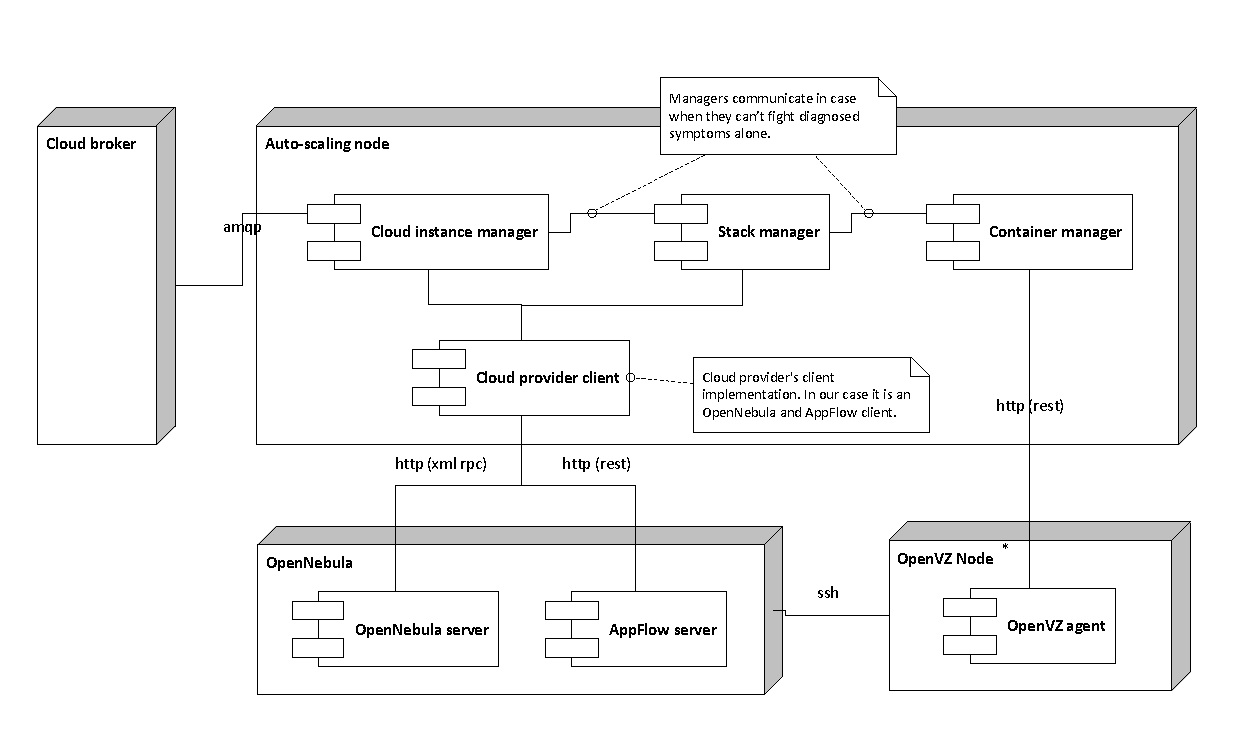
\includegraphics[width=\textwidth]{chapter-implementation/auto-scaling-subsystem-deployment}
  \end{center}
  \caption{Deployment diagram of auto-scaling subsystem}
  \label{fig:auto-scaling-subsystem-deployment}
\end{figure}



\subsection{Container manager}

\subsubsection{Objectives}
\subsubsection{Implementation details}
\subsubsection{Control loop iteration}


\subsection{Stack manager}

\subsubsection{Objectives}
\subsubsection{Implementation details}


\subsection{Cloud instance manager}

\subsubsection{Objectives}
\subsubsection{Implementation details}


\section{Cloud provider}

\section{Exemplary scenarios}

\subsection{Service deployment}

\subsection{Scaling application}

\subsection{Scaling application across multiple cloud providers}

\section{Summary}

